\documentclass{article}

\usepackage{color}
\usepackage{graphicx}
\usepackage{tabularx}


\usepackage{geometry,wrapfig,lipsum}
 \geometry{
 top=20mm,
 bottom=20mm,
 }


\title{Document pour l'adapation des interfaces}
\author{Justal Kevin}
\date{28/09/2015}
\renewcommand{\contentsname}{Table des mati\`eres} 
 
\newcommand\invisiblesection[1]{%
  \refstepcounter{section}%
  \addcontentsline{toc}{section}{\protect\numberline{\thesection}#1}%
  \sectionmark{#1}} 
 
\begin{document}

\begin{center}
\textbf{\Huge{JEU DES COULEURS}}
\line(1,0){300}\\
ANALYSE ET TEST APPROFONDIS\\
\vspace{3cm}
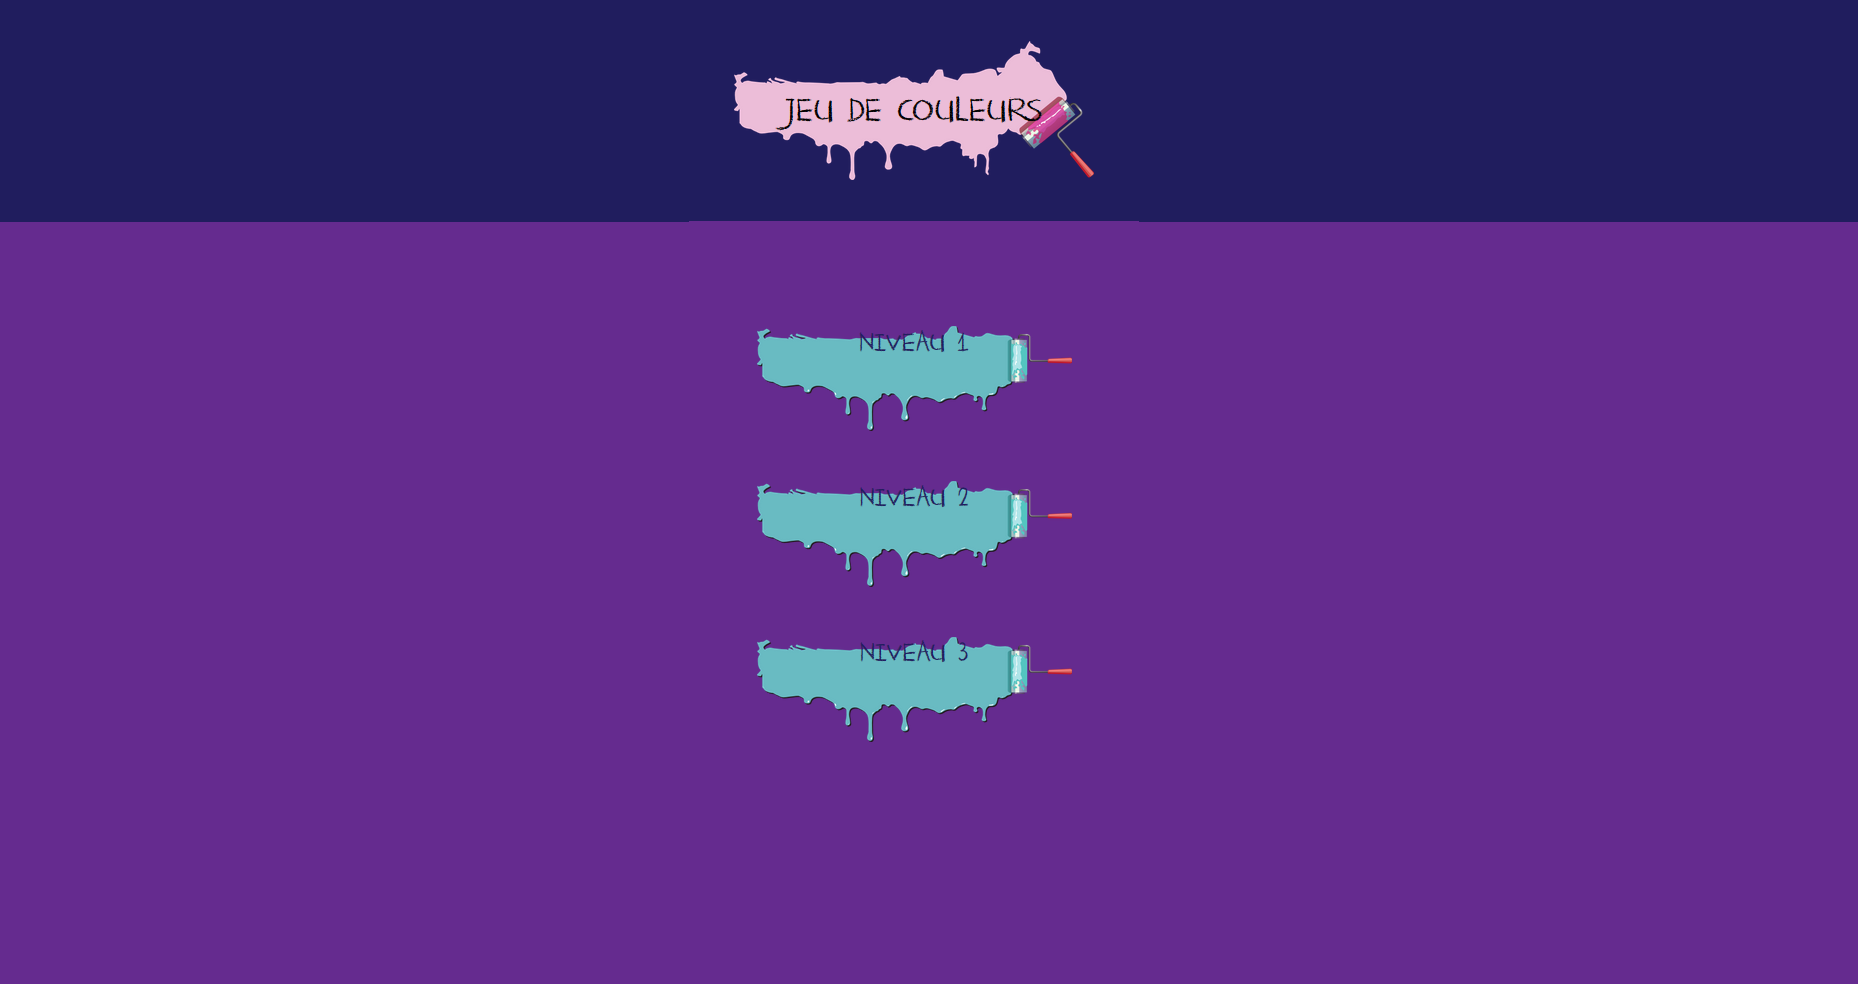
\includegraphics[width=\textwidth]{2}\\
\vspace{3cm}
\textbf{\Large{JUSTAL KEVIN}}\\
2015\\
\vspace{2cm}
\textbf{Justal Kevin - \color{blue}{\underline{justal@polytech.unice.fr}} \color{black}{- SI5 - IHM}}\\
\vspace{4cm}
\textbf{Enseignant :}\\
\textbf{Jean-Paul Stromboni - \color{blue}{\underline{strombon@polytech.unice.fr}}}
\end{center}

\newpage
\tableofcontents

\newpage

\section{Qualit\'es}

\vspace{0.5cm}

\includegraphics[width=\textwidth]{4}\\
\hspace*{0.6cm}La qualit\'e du jeu r\'eside dans son gameplay tr\`es simple et intuitif. Il n'y rien d'extravagant sur l'\'ecran qui perturberait le joueur. Il y a juste le minimum pour que le jeu soit jouable, c'est \`a dire 3 couleurs, 3 pot de peinture et 3 t\^aches. On comprend donc tr\'es vite le principe du jeu. Les t\^aches doivent aller dans leurs pots de peinture respective. Un autre bon point pour le jeu est la vitesse d'\'execution du programme ainsi que le peu de ressources utilis\'es. Le jeu doit charger environs 280,83 ko, ce qui est une valeur relativement faible pour un jeu.\\

\begin{wrapfigure}{l}{0.2\textwidth}
  \vspace{-20pt}
  \begin{center}
    
\includegraphics[width=0.18\textwidth]{10}
  \end{center}
  \vspace{-20pt}
  \caption{Le curseur du drag and drop}
  \vspace{-10pt}
\end{wrapfigure}

\hspace*{0.6cm}La prise en main est simple car le "drag and drop" du jeu est tr\`es bien con\c{c}u. Il y a deux mani\`eres de le manipuler. De mani\`ere classique, on peux effectuer simplement un glisser-d\'eposer. On prend la t\^ache de peinture puis on la d\'eplace dans le pot correspondant. Mais j'ai appris lors de ma visite \`a l'IME (Institute M\'edico Educatif) Hirondelles de Biot que les utilisateurs avaient g\'en\'eralement du mal \`a garder le clic appuy\'e. C'est pourquoi on trouve dans ce jeu, une deuxi\`eme mani\`ere d'\'effectuer la m\^eme op\'eration en cliquant sur la t\^ache puis sur le pot de peinture. Ceci est une tr\`es bonne id\'ee que je vais sans doute reprendre pour mon propre projet.\\

\begin{wrapfigure}{r}{0.2\textwidth}
  \vspace{-20pt}
  \begin{center}
    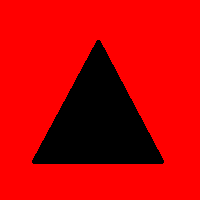
\includegraphics[width=0.18\textwidth]{5}
  \end{center}
  \vspace{-20pt}
  \caption{Symbole lorsque l'on perd}
  \vspace{-10pt}
\end{wrapfigure}

\hspace*{0.6cm}La situation du joueur est aussi tr\`es bien d\'ecrite dans le jeu. Lorsque le joueur triomphe du jeu ou perd, un symbole visuel apparait et un son est jou\'e. Cela est une tr\`es bonne id\'ee. Le jeu vise ainsi un public plus large. Les d\'eficients visuels peuvent ainsi entendre lorsqu'il font une erreur, il n'ont pas besoin de voir le symbole affich\'e sur l'\'ecran. De m\^eme pour les sourds, le symbole qu'ils voient est suffisamment intuitif pour comprendre si la r\'eponse est juste ou non.\\

\newpage

\section{D\'efauts}

\begin{wrapfigure}{l}{0.3\textwidth}
  \vspace{-20pt}
  \begin{center}
    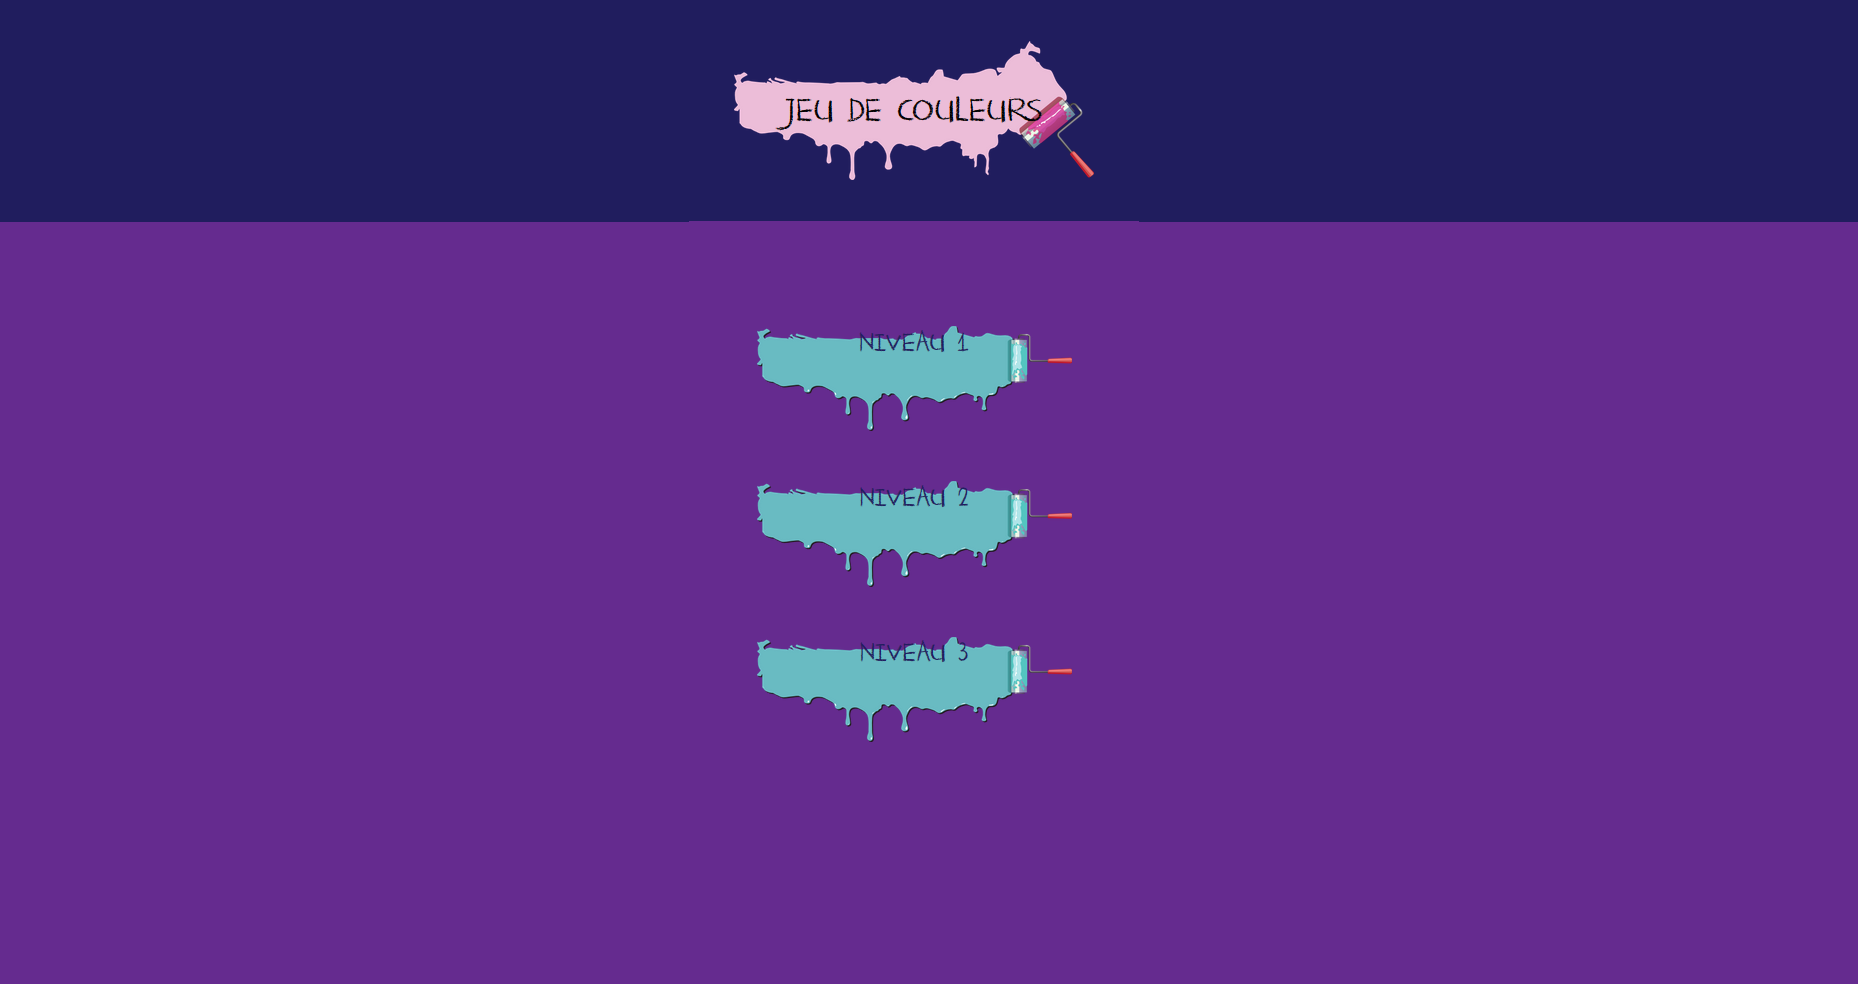
\includegraphics[width=0.28\textwidth]{2}
  \end{center}
  \vspace{-20pt}
  \caption{Menu difficilement lisible}
  \vspace{-10pt}
\end{wrapfigure}
\hspace*{0.6cm}Le menu principal n'utilise pas tout l'espace disponible, \`a certaines tailles d'\'ecran il devient difficile de lire le menu. Moi-m\^eme qui n'ai qu'un l\'eger probl\^eme de vue doit me forcer un peu pour lire le menu. La couleur, la taille ainsi que la police ont \'et\'e tr\`es mal choisis. La couleur du texte est noir et repose sur un petit rectangle de couleur claire. Cependant tout le reste du fond est violet fonc\'e. Il n'y a pas assez de contraste pour rendre le menu visible pour les malvoyants.\hfill\\

\`A l'int\'erieur du jeu, il n'y a pas de grande faute majeur. Seulement de petit d\'etail qui aurait pu \^etre \'evit\'e et ainsi am\'elior\'e l'exp\'erience de l'utilisateur. Par exemple, le clic droit aurait pu \^etre d\'esactiv\'e pour \'evit\'e aux utilisateurs de faire un clic droit maladroit et se retrouver dans les menus du navigateur internet. Notons aussi que dans le niveau 2, il est possible de sortir les \'el\'ements de l'\'ecran. Sur tablette, en faisant un mauvais mouvement, on peux donc se retrouver avec un \'el\'ement hors de l'\'ecran, le jeu en devient donc fig\'e.\\
\begin{wrapfigure}{r}{5cm}
\vspace{6pt}
\centering
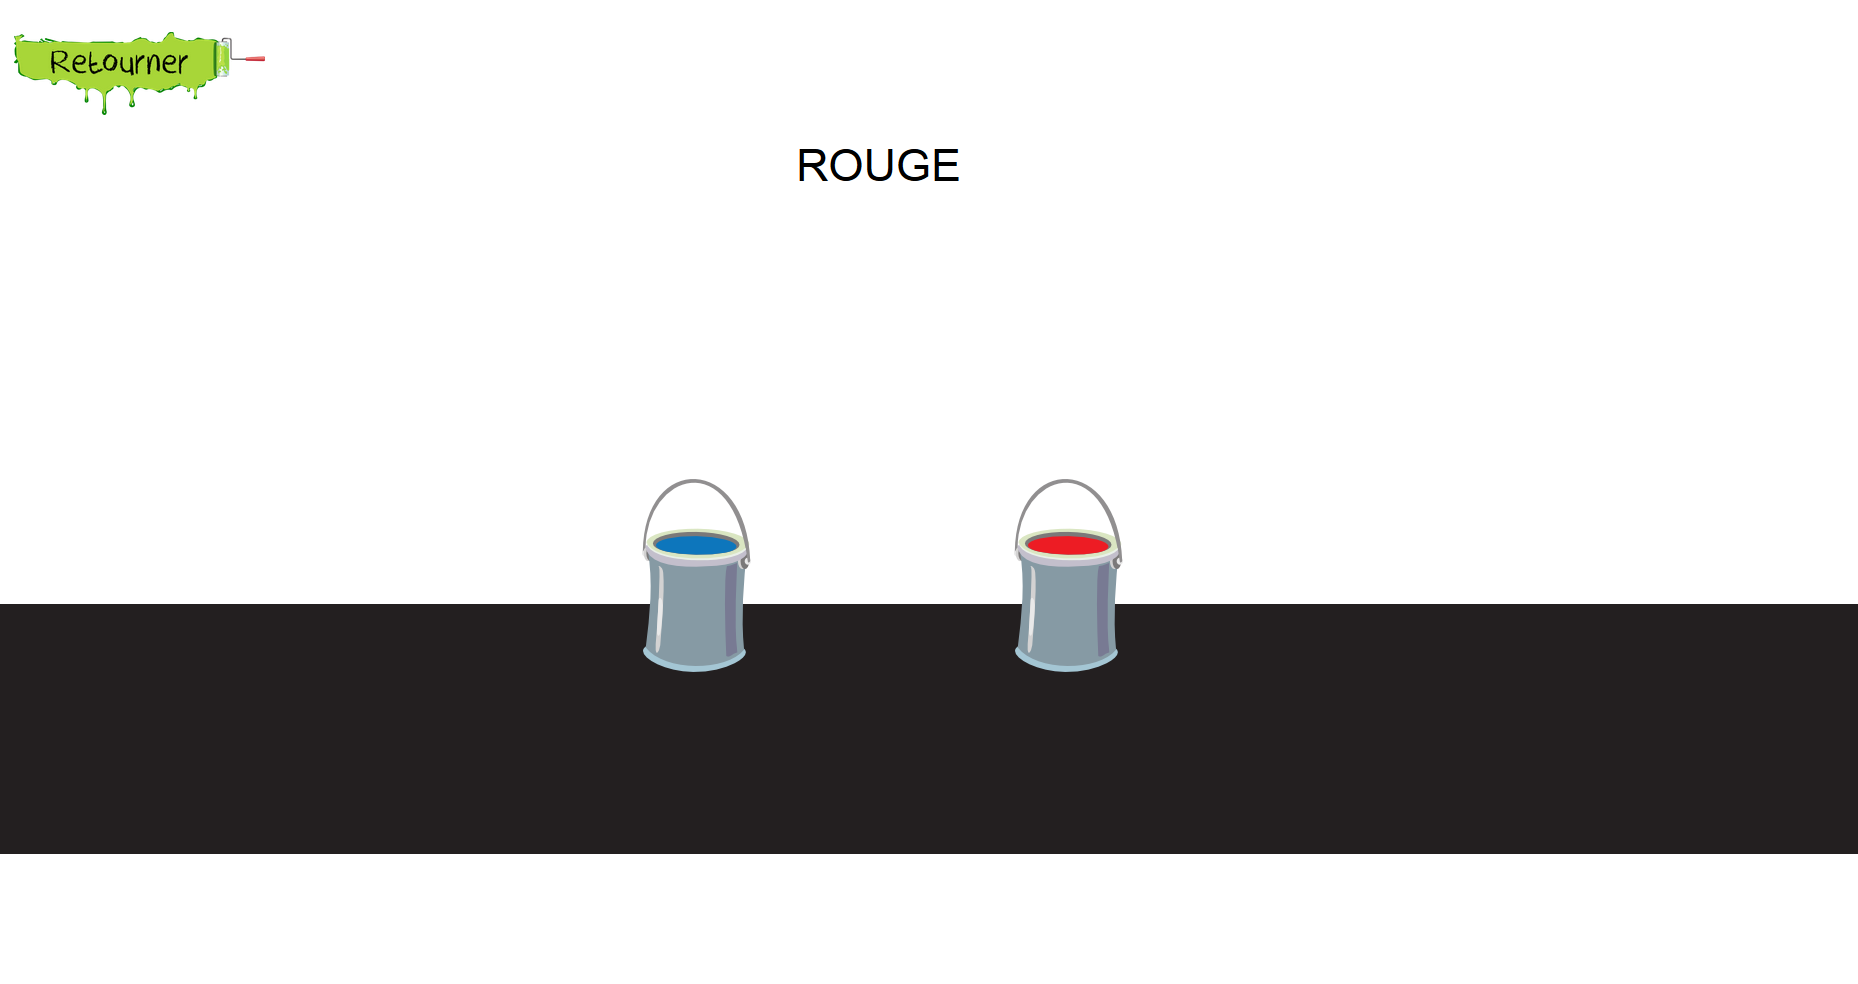
\includegraphics[width=5cm]{6}
\end{wrapfigure}
{\hspace*{0.6cm}Sur le niveau 3, il y a un gros probl\`eme d'interf\'erence. Nous sommes en plein dans l'effet Stroop. Cette notion du domaine psychologique pr\'ecise que notre temps de r\'eaction et pourcentage d'erreurs augmentent lorsqu'il y a des information \`a filtrer. Inconsciemment, notre cerveau va lire la couleur affich\'e puis lire le mot. La couleur de ce niveau est marqu\'e en noir. L'utilisateur va donc toujours penser \`a la couleur du texte en premier. Ensuite, l'utilisateur lira le mot et comprendra qu'il faut prendre tel ou tel autre couleur.}
\vspace{0.5cm}\\
Il n'est pas si \'evident de lire le nom d'une couleur \'ecrite avec une couleur diff\'erente. Il aurait mieux fallut associer la couleur du texte \`a la couleur \'ecrite. Par exemple, une am\'elioration possible serait d'\'ecrire en rouge, le mot rouge.

\newpage

\begin{center}
\vspace{0.5cm}
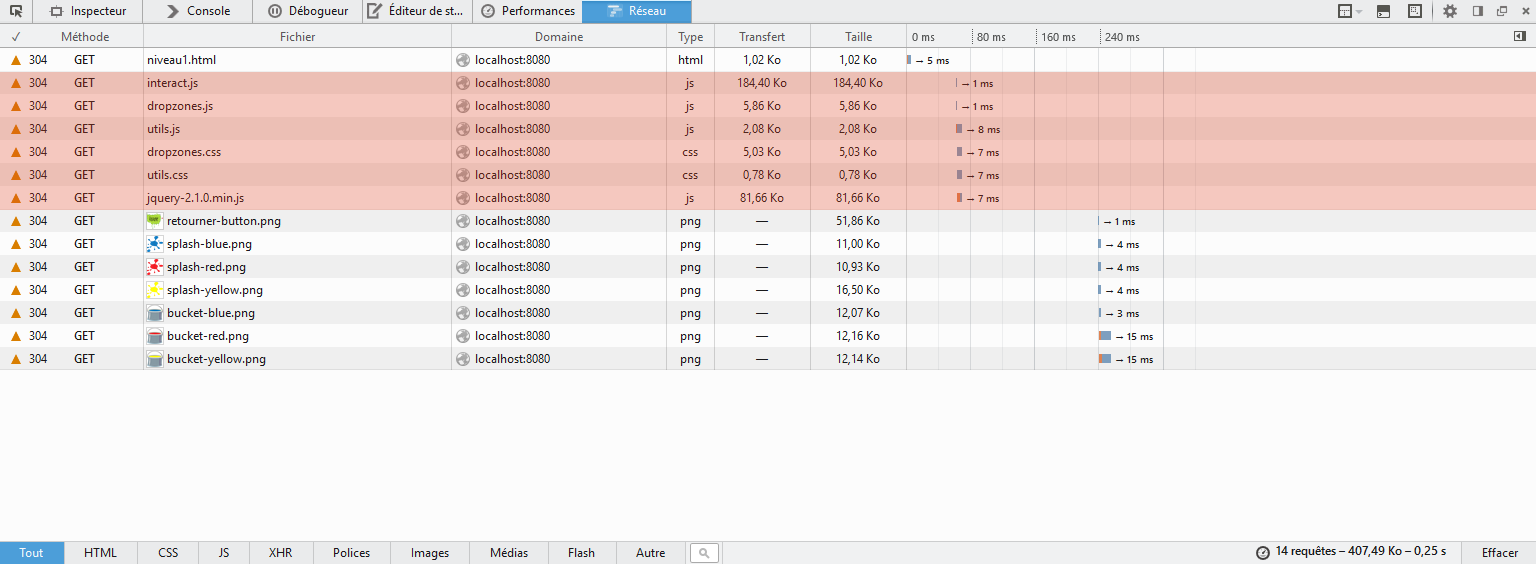
\includegraphics[width=\textwidth]{7}\\
\end{center}

Il y a aussi un point n\'egative dans l'ordre d'\'ex\'ecution des ressources. Comme on peux le voir sur l'image ci-dessus qui est une analyse sous Firebug, les scripts sont charg\'es avant les images. Pour am\'eliorer ce point, il aurait fallu mettre les scripts \`a la fin dans le code HTML et non au d\'epart. 

\begin{center}
\vspace{0.5cm}
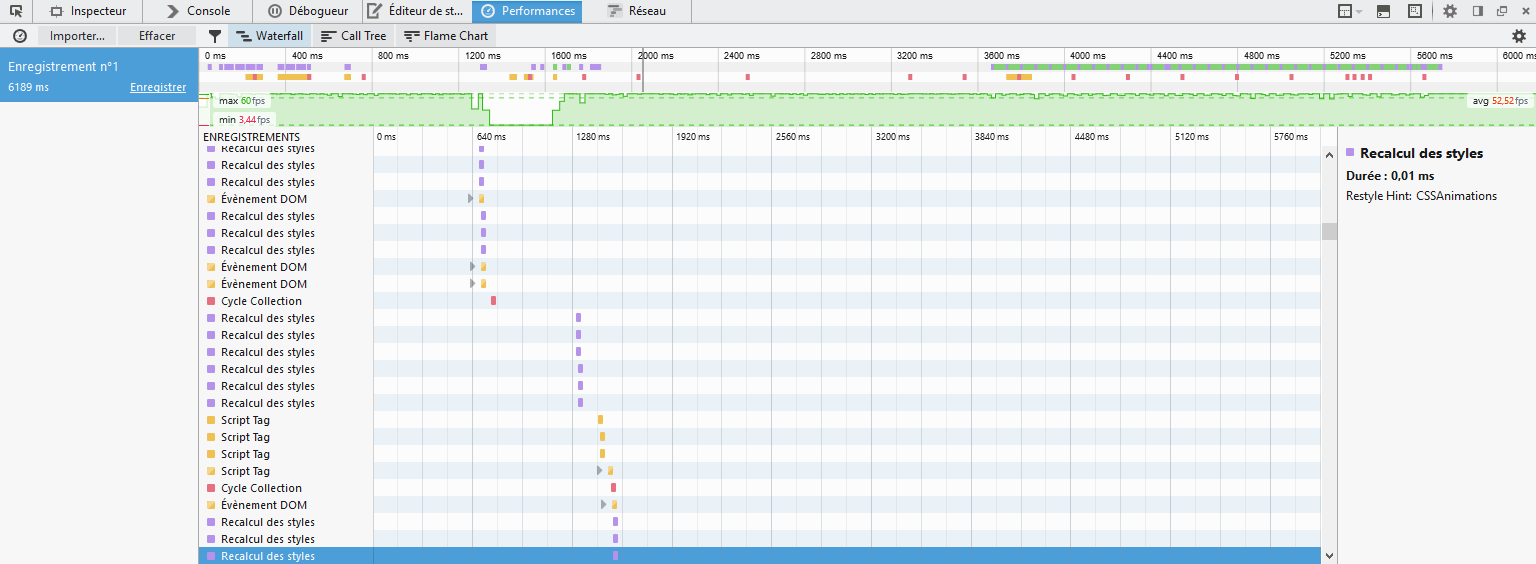
\includegraphics[width=\textwidth]{8}\\
\end{center}

Toujours dans Firebug, une autre chose est pr\'eoccupante. Sur l'image ci-dessus, on remarque que les FPS (Frames per second/Images par seconde) moyen ne sont qu'\`a 52. Pour un tel jeu, il est \'etonnant que ce chiffre ne soit pas \'egale \`a la fr\'equence de l'\'ecran, soit 60 FPS. \\
On remarque que le jeu subit une chute de FPS \`a 3 FPS apr\`es 1,2 secondes de chargement de la page et jusqu'\`a 1,6 secondes. Plusieurs erreurs mineurs ralentissent le jeu ainsi que le "cycle collector" du navigateur, c'est \`a dire la recherche des ressources dans le dossier temporaire du navigateur. Pour un tel jeu o\`u les ressources sont minuscules, il aurait \'et\'e sans doute plus efficace de forcer le navigateur \`a ignorer cet \'etape.

\newpage

\section{Programmation}

\hspace*{0.6cm}Du cot\'e programmation, il y a l\`a aussi plusieurs probl\`emes plus ou moins emb\'etant. Premi\`erement, un code finit ne devrais jamais contenir de code comment\'e, c'est une mauvaise pratique. Cela peut avoir de grave cons\'equence lors d'un d'une recherche de bug. Deuxi\`emement, le code contient du "dead code", c'est \`a dire du code qui ne sera jamais atteint ou qui ne servira jamais peut importe ce qu'il contient. Par exemple, dans le niveau 1, on retrouve une balise "script" vide et apr\`es la balise "html".

\vspace{0.4cm}
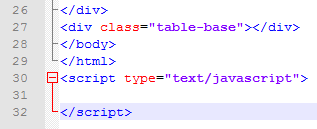
\includegraphics[width=0.40\textwidth]{9}\\

La seconde chose \`a not\'e est l'utilisation tr\`es mauvaise des attributs CSS. Cette mauvaise manipulation rend le jeu inadapt\'e sur certains \'ecran.\\
\begin{wrapfigure}{r}{5cm}
\vspace{-13pt}
\centering
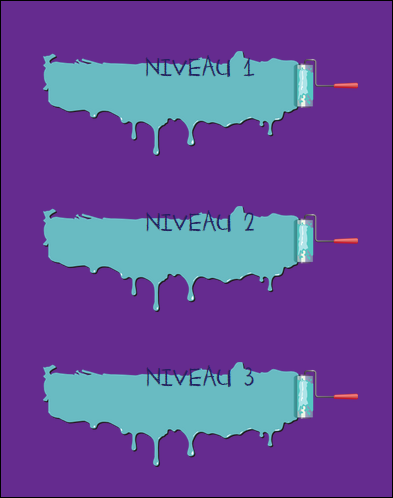
\includegraphics[width=5cm]{1}
\caption{\textit{\`A certaines dimensions d'\'ecrans, le texte sort du graphisme.}}
\end{wrapfigure}
{\hspace*{0.6cm}Il s'agit l\`a d'une des permi\`eres erreurs qui m'a simplement saut\'e aux yeux. Mon \'ecran \'etant relativement grand par rapport \`a la moyenne, je remarque g\'en\'eralement tr\`es rapidement si un site ou un jeu s'adapte ou non \`a l'\'ecran de l'utilisateur. Ici, comme on peux le voir sur l'image de droite, le jeu ne s'adapte pas du tout \`a tous les utilisateurs. L'erreur a \'et\'e assez simple \`a trouver, il s'agit d'une incompr\'ehension des \'etudiants sur l'attribut CSS "padding" et "margin". Il fallait tout simplement utiliser le padding \`a la place du margin dans les balises divisions "option". Sans cela, la balise "div" qui \'etait contenue dans la balise "a" se retrouvait tout simplement \`a une taille diff\'erente de la balise "a" qui l'entourait. Cette erreur se reproduit sur les 3 liens vers les diff\'erents niveaux.}\\

Il y a aussi une utilisation tr\`es mauvaise des balises "div" ou une m\'econnaissance inqui\'etante de certains attributs fondamentales de CSS.\\

\hfill
\begin{wrapfigure}{l}{3.9cm}
\vspace{-13pt}
\centering
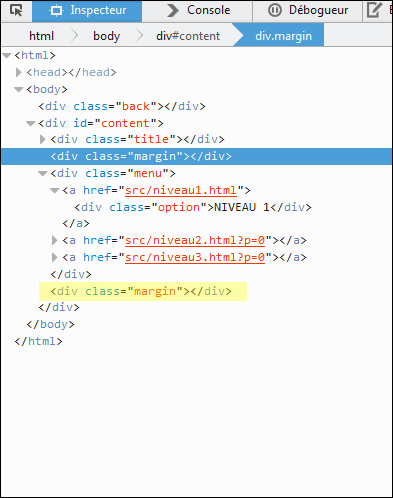
\includegraphics[width=3.9cm]{3}
\caption{\textit{Mauvais code \'etudi\'e sous Firebug}}
\end{wrapfigure}
{\hspace*{0.6cm}Le rectangle jaune sur l'image de gauche pointe sur un probl\`eme s\'erieux de programmation, les \'el\`eves responsables de ce code ont util\'e des balises "div" pour effectuer des marges et ainsi r\'ealiser le positionnement de leurs \'el\'ements HTML. Ceci est consid\'er\'e comme une tr\`es mauvaise pratique. Pour r\'ealiser le positionnement, il est plus int\'eressant d'utiliser les attributs CSS tels que "position","display","float","margin","padding"... On peux de plus not\'e que les \'el\`eves n'ont aussi pas respect\'e les normes du W3C (World Wide Web Consortium). Il est non conforme d'englob\'e une balise "block" comme une "div" dans une balise "inline" comme un "a". Pour regler ce probl\`eme, il fallait soit faire de la balise "div" un lien vers la page en utilisant JavaScript ou alors transformer l'attribut "display" de la balise "div" en "inline" ou "inline-block".}\\

\newpage

\section{Am\'elioration}

\hspace*{0.6cm}J'ai d\'ej\`a propos\'e aux travers de mon document plusieurs am\'eliorations, je vais donc les regrouper ici et en compl\'etant cette liste avec d'autres id\'ees :\\
\begin{itemize}
  \item Mettre un bouton ou une indication que le jeu au niveau 1 montre le gameplay et qu'il n'y a rien \`a faire.
  \item Am\'eliorer la visibilit\'e du texte au menu
  \item Mettre le texte de la m\^eme couleur que celle \'ecrite dans le niveau 3.
  \item D\'esactiver le clique droit pour \'eviter que l'utilisateur ne rentre dans les menus de son navigateur.
  \item Mettre une limite au d\'eplacement possible des \'el\'ements dans le niveau 2, sinon on peux bloquer le jeux en sortant un \'el\'ement de l'\'ecran.
  \item Rendre le jeu compatible avec tous les navigateurs (Le jeu ne fonctionne pas sous Safari)
  \item Ajouter les couleurs compl\'ementaires (rose,orange..)
  \item Mettre une option permettant d'ajouter ou d'enlever des pots de peintures.
\end{itemize}


\end{document}
